\documentclass{standalone}
%
\usepackage{tikz}
\usetikzlibrary{backgrounds,shapes.callouts}
\usepackage{tkz-euclide}
\usepackage{xcolor}
%\usepackage{pgfplots}
%\usepackage{freetikz}
%\usetikzlibrary{shapes}
%\definecolor{eduinafred}{HTML}{BB2D58}
%\definecolor{eduinafblu}{HTML}{1D71B8}
%
\definecolor{space}{HTML}{0A2543}
\definecolor{mercury}{HTML}{846549}
\definecolor{venus}{HTML}{BB9765}
\definecolor{earth}{HTML}{0089FA}
\definecolor{mars}{HTML}{DC7B4E}
\definecolor{jupiter}{HTML}{A79476}
\definecolor{saturn}{HTML}{DBBD9B}
\definecolor{saturnring}{HTML}{857C73}
\definecolor{uranus}{HTML}{b1d8dd}
\definecolor{neptune}{HTML}{799bc1}
\definecolor{pluto}{HTML}{ceaa8a}
\definecolor{dida}{HTML}{FFDE00}
\definecolor{title}{HTML}{FBA706}
%
%\definecolor{glasses}{HTML}{08663D}
\definecolor{moon}{HTML}{AFAFAF}
%\definecolor{craterm}{HTML}{616060}
%\definecolor{linem}{HTML}{DBDBDB}
%\definecolor{core3}{HTML}{FFD016}
%
\usepackage{fontspec}
\setmainfont{Open Dyslexic}
%\setmainfont{Montserrat Medium}
%
\title{Sistema Solare}
\begin{document}
	\tikzset{
		partial ellipse/.style args = {#1:#2:#3}{insert path={+ (#1:#3) arc (#1:#2:#3)}},
		notice/.style  = { draw, ellipse callout, callout relative pointer={#1} },
	}
	\begin{tikzpicture}[background rectangle/.style={fill=white},show background rectangle,>={[inset=0,angle'=27]Stealth}]
		\def\rsun{1}
		\def\rmer{0.2}
		\def\rven{0.5}
		\def\ret{0.53}
		\def\rmn{0.2}
		\def\rms{0.28}
		\def\rj{1}
		\def\rsat{1}
		\def\rur{1}
		\def\rnp{1}
		\def\rp{0.1}
		%
		\def\d{2}
		%
		\draw [use as bounding box] (-20,20) -| (20,20) |- (20,-76) -| (-20,-76);
		%title
		\begin{scope}
			\draw [black,ultra thick,fill=title] (-18,18.5) rectangle (18,11.5);
			\node (example-textwidth-2) [align=center, text width=40cm, color=black, font=\fontsize{90pt}{91pt}\selectfont] at (0,15) {Il sistema ticonico};
		\end{scope}
		%
		\begin{scope}[shift={(-10,7)}]
			\node at (23,0) {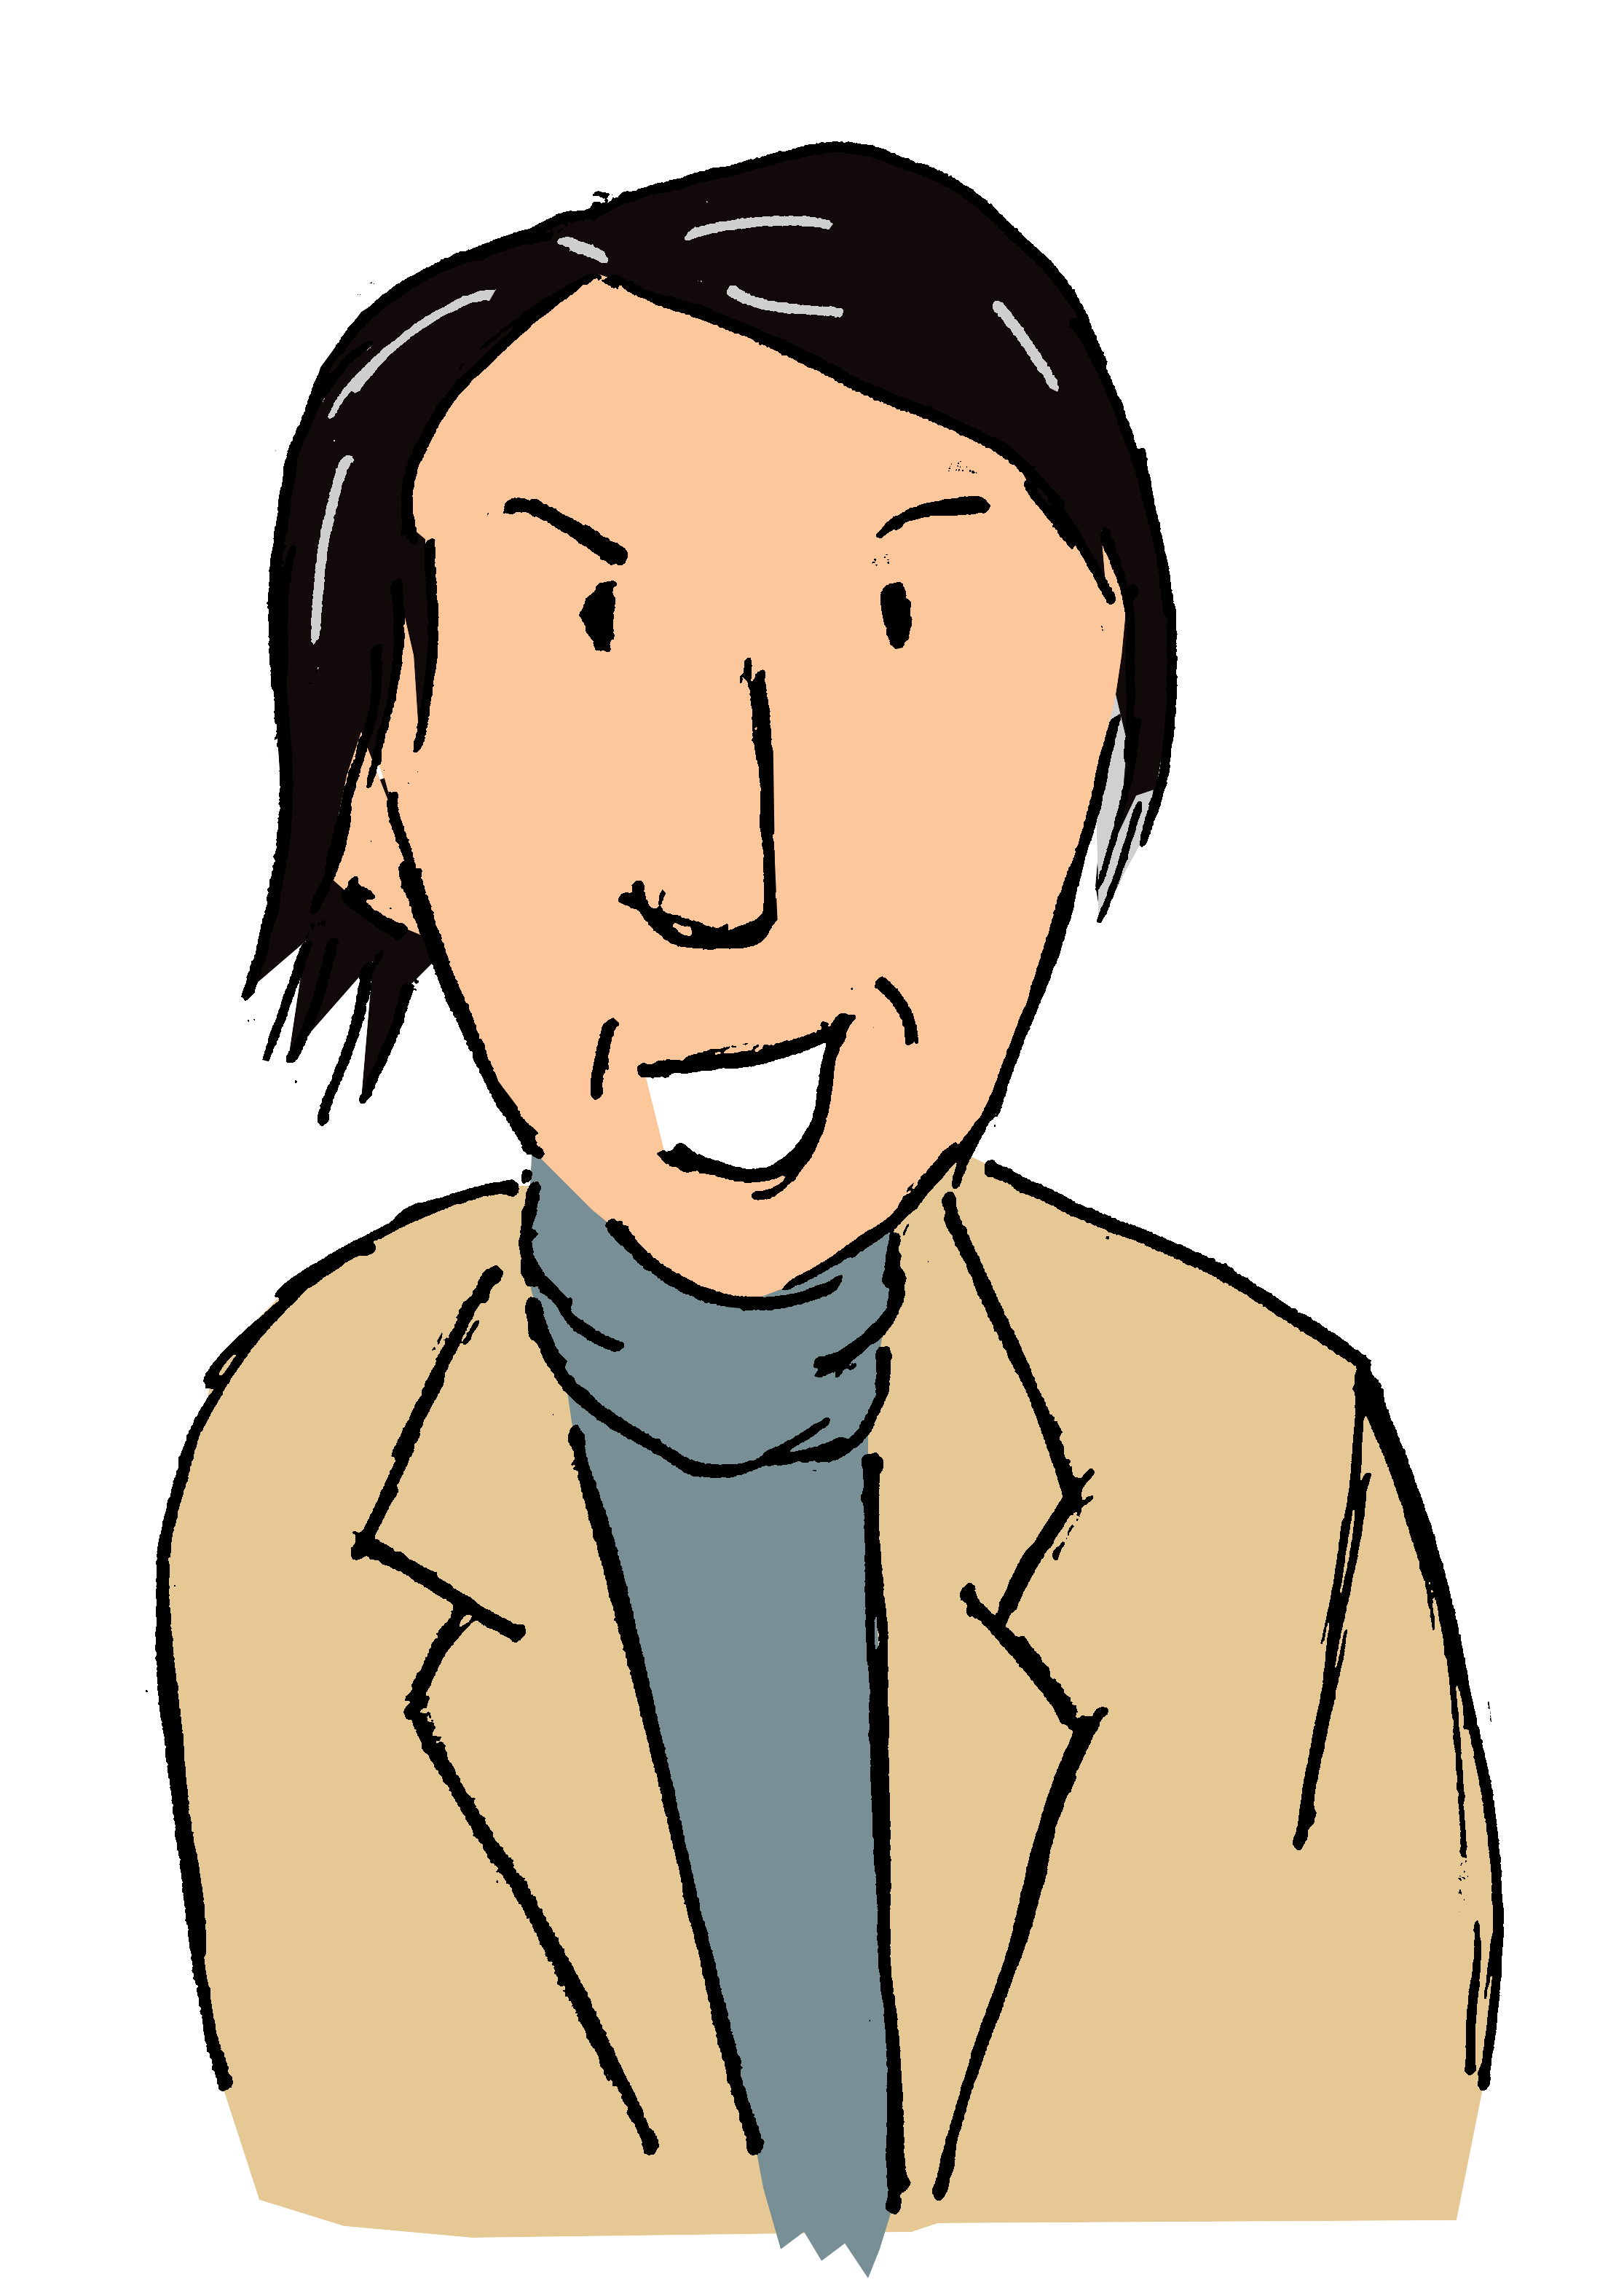
\includegraphics[width=5cm]{img/carl_sagan}};
			\node (example-textwidth-2) [notice={(3,0.5)}, ultra thick, right, align=center, text width=12cm, color=black, fill=white, font=\fontsize{23pt}{24pt}\selectfont] at (1,-1) {Il primo a rivoluzionare il modello tolemaico fu \textbf{Tycho Brahe} che, riprendendo un'idea di \textbf{Marziano Capella}, propose una struttura che consentiva di abbandonare gli epicicli.};
		\end{scope}
		%
		\begin{scope}[shift={(-3,-15)}]
			\draw [fill=space] (-14,15) rectangle (20,-15);
			\tkzDefPoint(0,0){E} %Earth
			\tkzDefShiftPoint[E](0.5*\d,0){L0} %Moon
			\tkzDefShiftPoint[E](2*\d,0){S0} %Sun
			\tkzDefShiftPoint[S0](0.5*\d,0){Mr} %Mercury
			\tkzDefShiftPoint[S0](0.7*\d,0){V0} %Venus
			\tkzDefShiftPoint[S0](4.5*\d,0){M0} %Mars
			\tkzDefShiftPoint[S0](5.3*\d,0){J0} %Jupiter
			\tkzDefShiftPoint[S0](6*\d,0){R0} %Saturn
			%
			\tkzDrawCircle[color=moon,ultra thick](E,L0)
			\tkzDrawCircle[color=white,ultra thick](E,S0)
			\tkzDrawCircle[color=mercury,ultra thick](S0,Mr)
			\tkzDrawCircle[color=venus,ultra thick](S0,V0)
			\tkzDrawCircle[color=mars,ultra thick](S0,M0)
			\tkzDrawCircle[color=jupiter,ultra thick](S0,J0)
			\tkzDrawCircle[color=saturn,ultra thick](S0,R0)
			%
			\tkzDefShiftPoint[E](0:\ret){E1}
			\tkzDrawCircle[color=black,ultra thick,fill=earth](E,E1)
			\tkzDefPointBy[rotation= center E angle -90](L0) \tkzGetPoint{l0}
			\node [above, xshift=2.2cm, text width=10cm, color=white, font=\fontsize{15pt}{16pt}\selectfont] at (E1) {Terra};
			%
			\tkzDefShiftPoint[l0](0:\rmer){L1}
			\tkzDrawCircle[color=black,ultra thick,fill=moon](l0,L1)
			\node [above, xshift=3cm, yshift=-0.5cm, text width=10cm, color=white, font=\fontsize{15pt}{16pt}\selectfont] at (L1) {Luna};
			%
			\tkzDefShiftPoint[S0](0:\ret){S1}
			\tkzDrawCircle[color=black,ultra thick,fill=white](S0,S1)
			\node [above, xshift=2.5cm, text width=10cm, color=white, font=\fontsize{15pt}{16pt}\selectfont] at (S1) {Sole};
			%
			\tkzDefShiftPoint[Mr](0:\rmer){mr}
			\tkzDrawCircle[color=black,ultra thick,fill=mercury](Mr,mr)
			\node [above, xshift=5.5cm, text width=10cm, color=white, font=\fontsize{15pt}{16pt}\selectfont] at (mr) {Mercurio};
			%
			\tkzDefPointBy[rotation= center S0 angle 110](V0) \tkzGetPoint{v0}
			\tkzDefShiftPoint[v0](0:\rmer){V1}
			\node [above, xshift=2.5cm, text width=10cm, color=white, font=\fontsize{15pt}{16pt}\selectfont] at (V1) {Venere};
			\tkzDrawCircle[color=black,ultra thick,fill=venus](v0,V1)
			%
			\tkzDefPointBy[rotation= center S0 angle 35](M0) \tkzGetPoint{m0}
			\tkzDefShiftPoint[m0](0:\rmer){M1}
			\tkzDrawCircle[color=black,ultra thick,fill=mars](m0,M1)
			\node [above, xshift=2.5cm, text width=10cm, color=white, font=\fontsize{15pt}{16pt}\selectfont] at (M1) {Marte};
			%
			\tkzDefShiftPoint[J0](0:\rmer){J1}
			\tkzDrawCircle[color=black,ultra thick,fill=jupiter](J0,J1)
			\node [above, xshift=2.5cm, text width=10cm, color=white, font=\fontsize{15pt}{16pt}\selectfont] at (J1) {Giove};
			%
			\tkzDefPointBy[rotation= center S0 angle -40](R0) \tkzGetPoint{r0}
			\tkzDefShiftPoint[r0](0:\rmer){R1}
			\tkzDrawCircle[color=black,ultra thick,fill=saturn](r0,R1)
			\node [above, xshift=2.5cm, text width=10cm, color=white, font=\fontsize{15pt}{16pt}\selectfont] at (R1) {Saturno};
			\draw [color=black,ultra thick] (-14,15) rectangle (20,-15);
		\end{scope}
		%
		\begin{scope}[shift={(-10,-32)}]
			\node at (23,0) {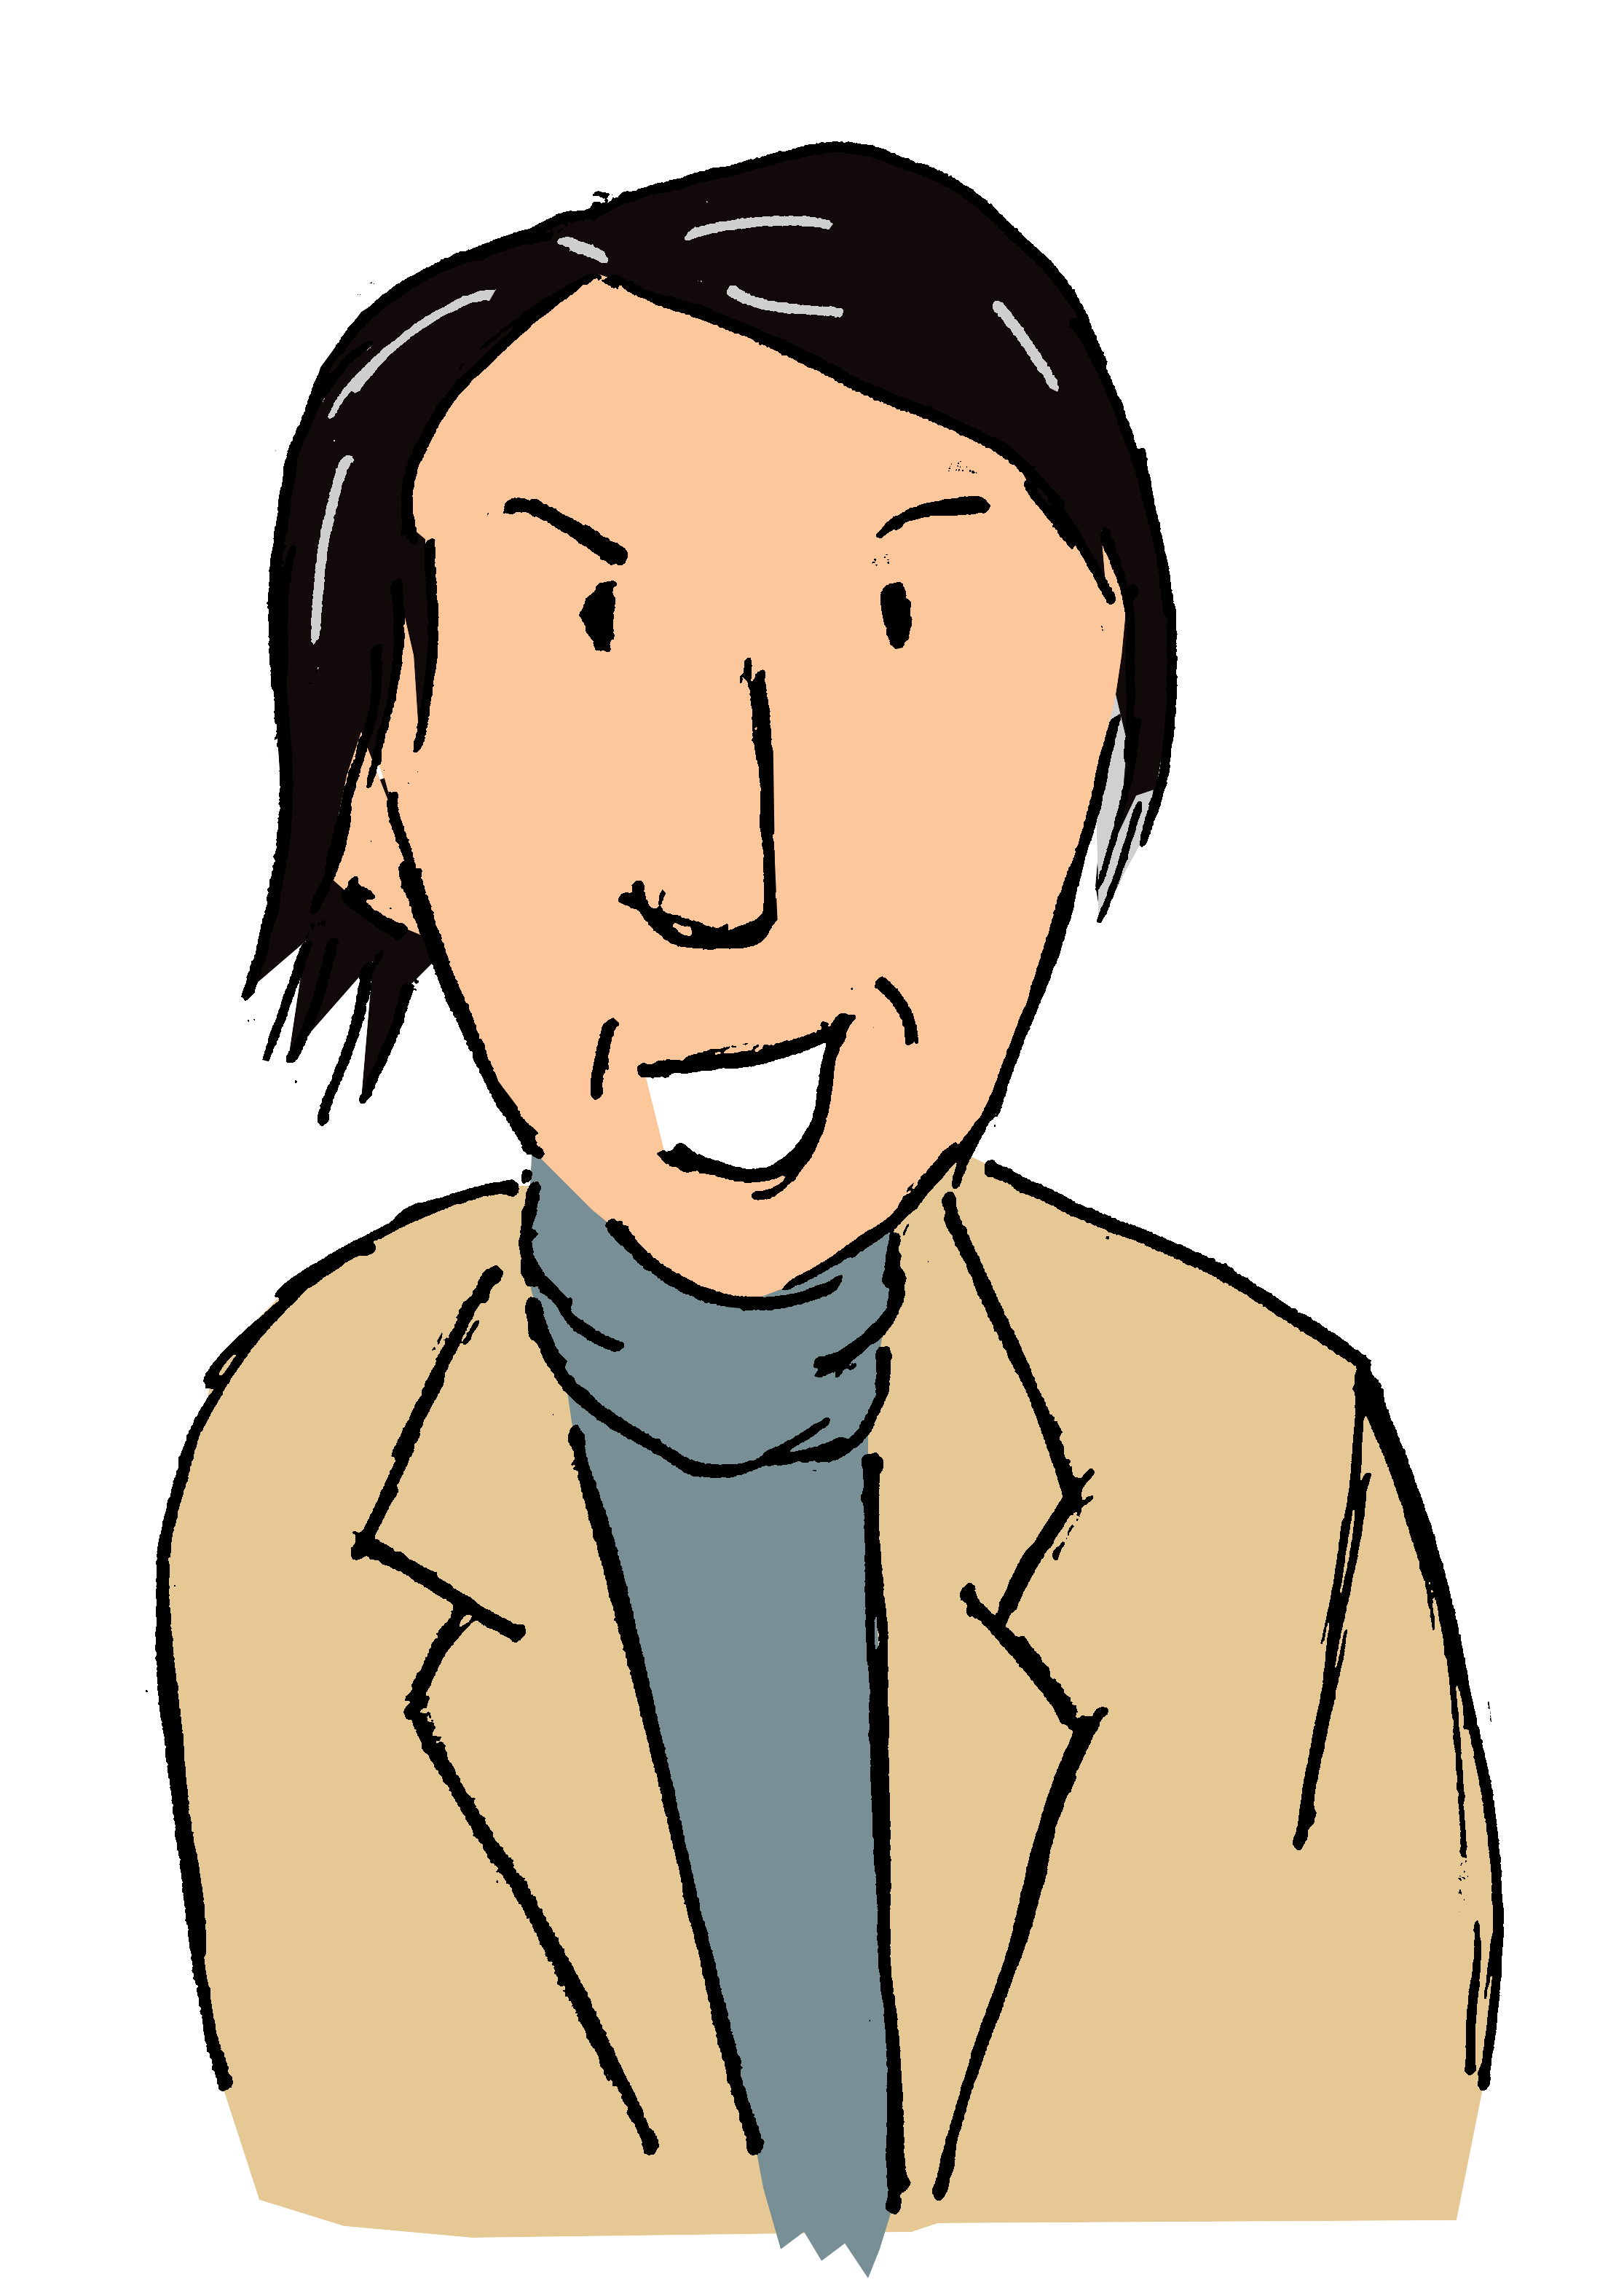
\includegraphics[width=5cm]{img/carl_sagan}};
			\node (example-textwidth-2) [notice={(2,0.5)}, ultra thick, right, align=center, text width=14cm, color=black, fill=white, font=\fontsize{23pt}{24pt}\selectfont] at (0.5,-1) {I vantaggi di questo modello furono essenzialmente due: la gran mole di osservazioni raccolte da Brahe e l'osservazione della fasi di Venere, non previste nel modello tolemaico.};
		\end{scope}
		%
		\begin{scope}[shift={(-10,-38)}]
			\node at (0,-2) {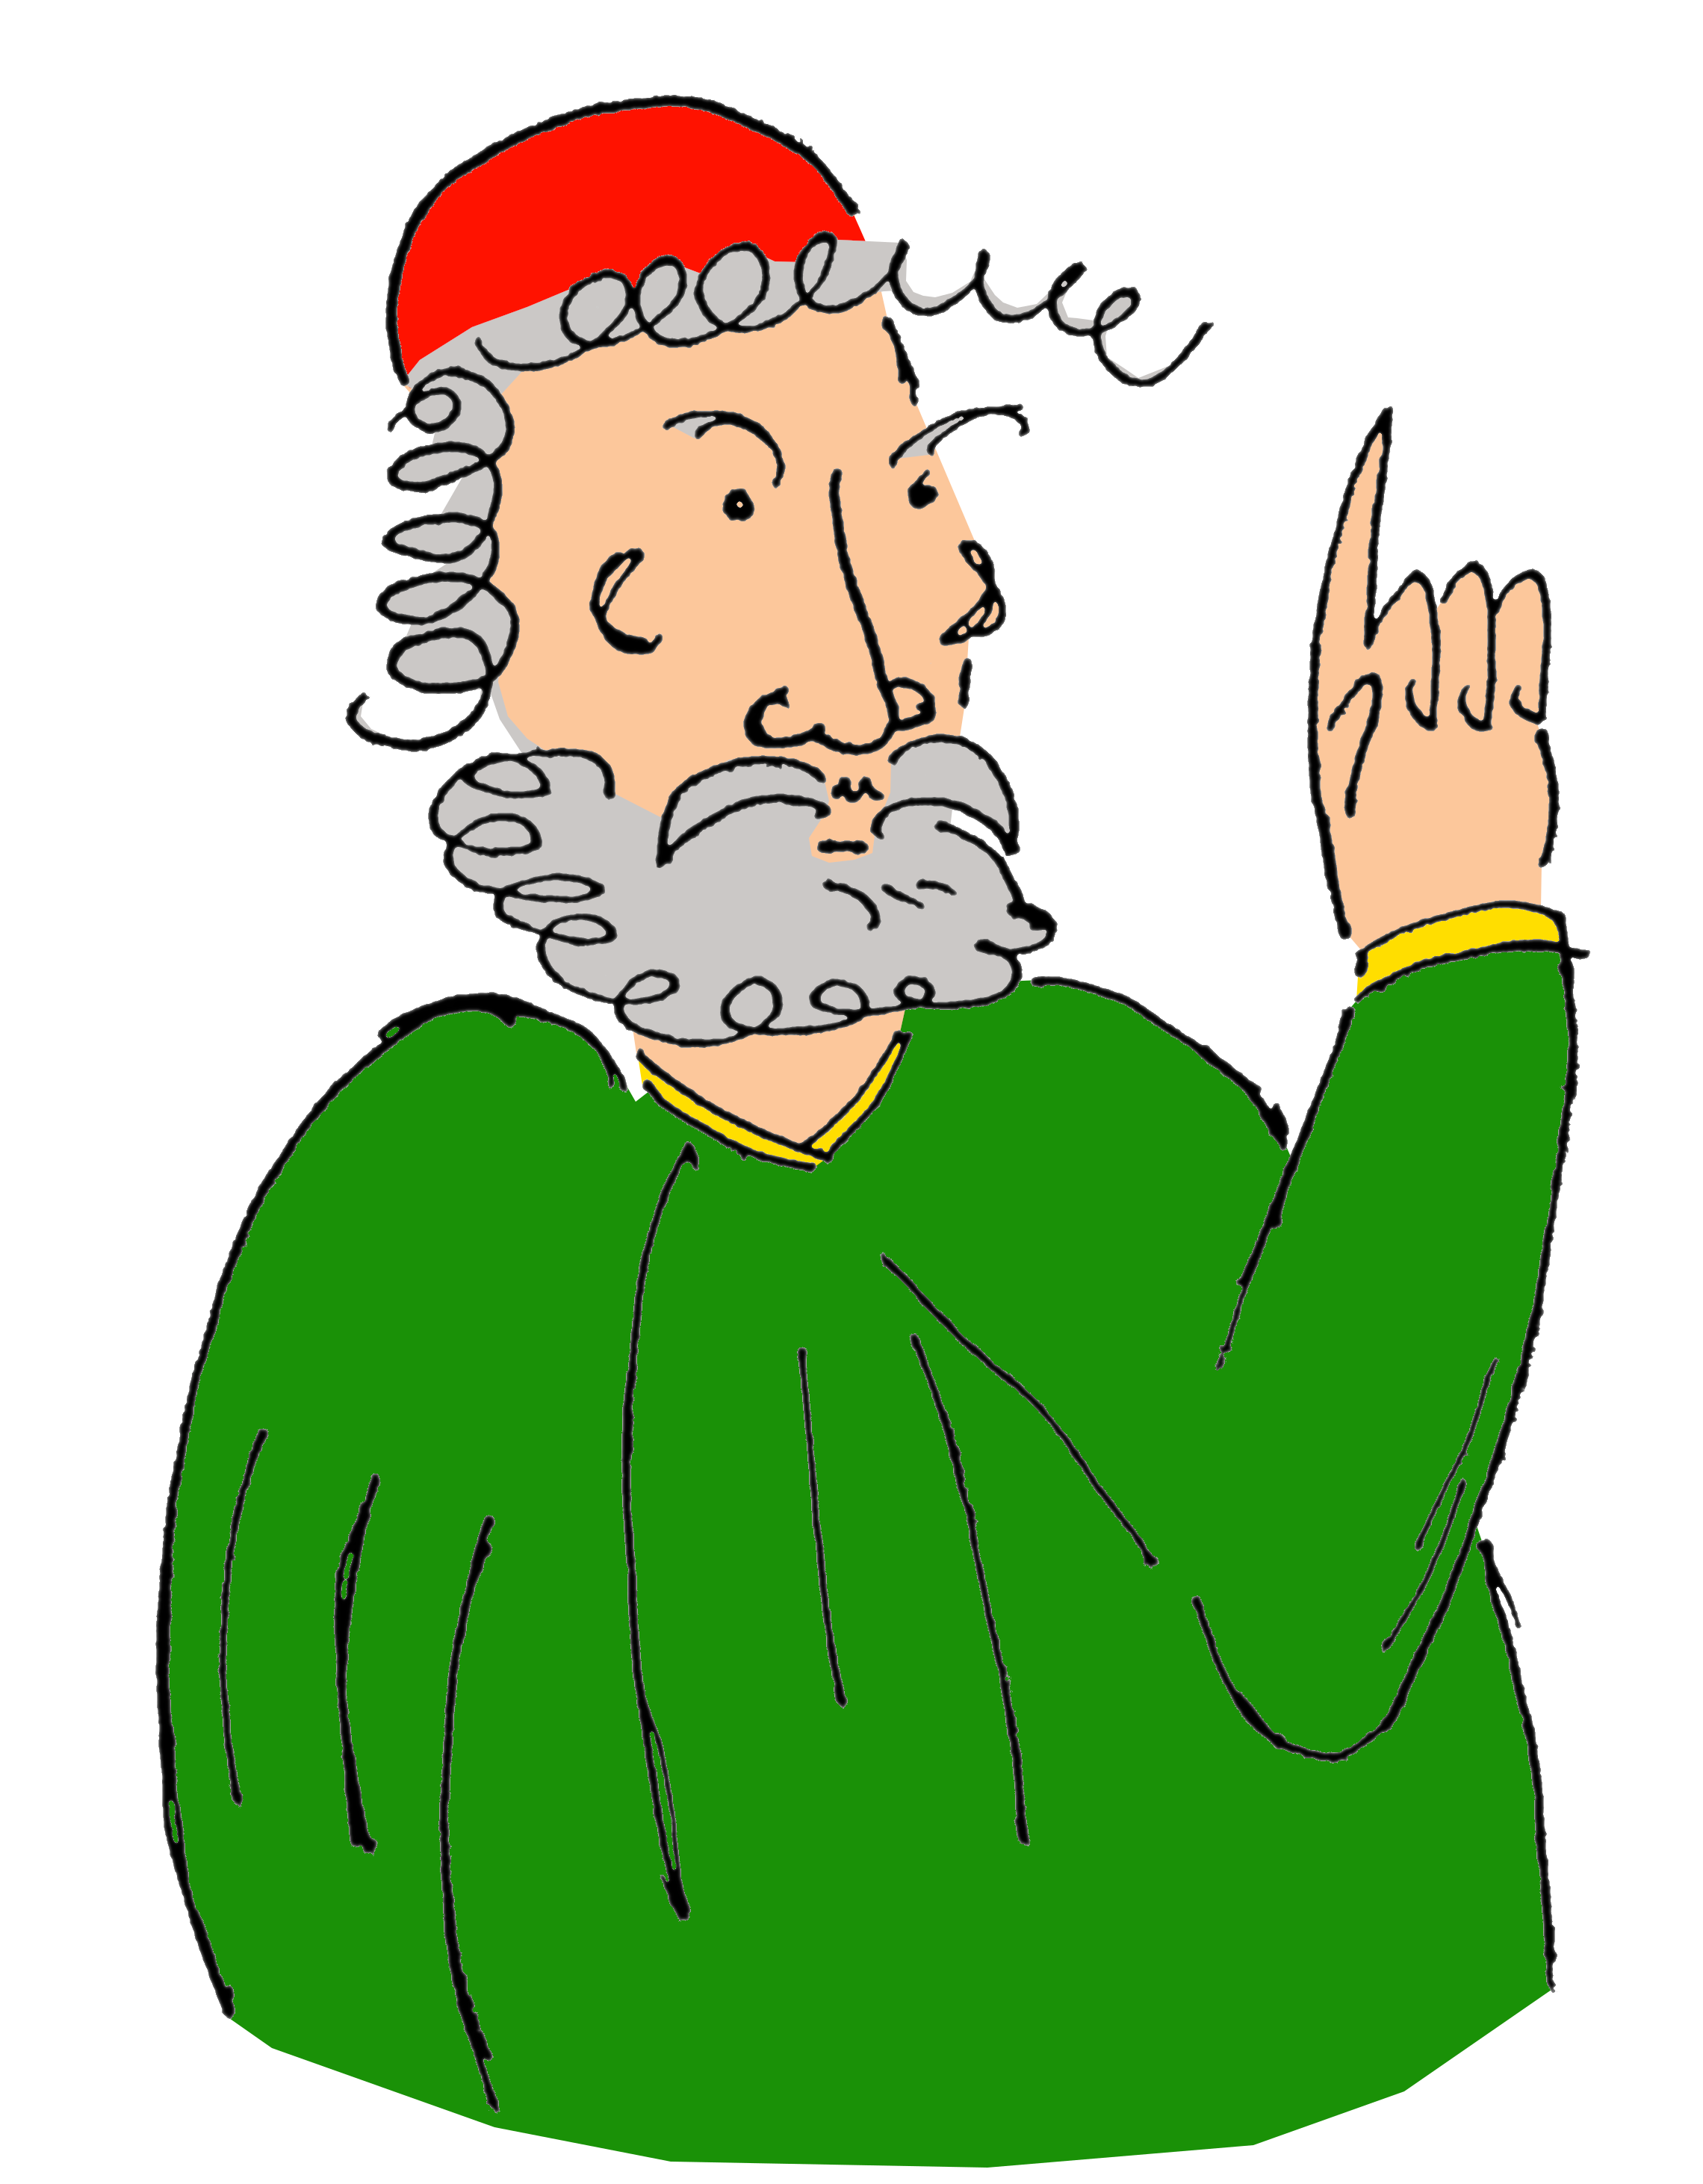
\includegraphics[width=6cm]{img/tolomeo}};
			\node (example-textwidth-2) [notice={(-3,1)}, ultra thick, right, align=center, text width=12cm, color=black, fill=white, font=\fontsize{23pt}{24pt}\selectfont] at (2,-4.5) {Non si puo' tenere conto di tutto!};
		\end{scope}
		%
		\begin{scope}[shift={(-10,-48)}]
			\node at (23,0) {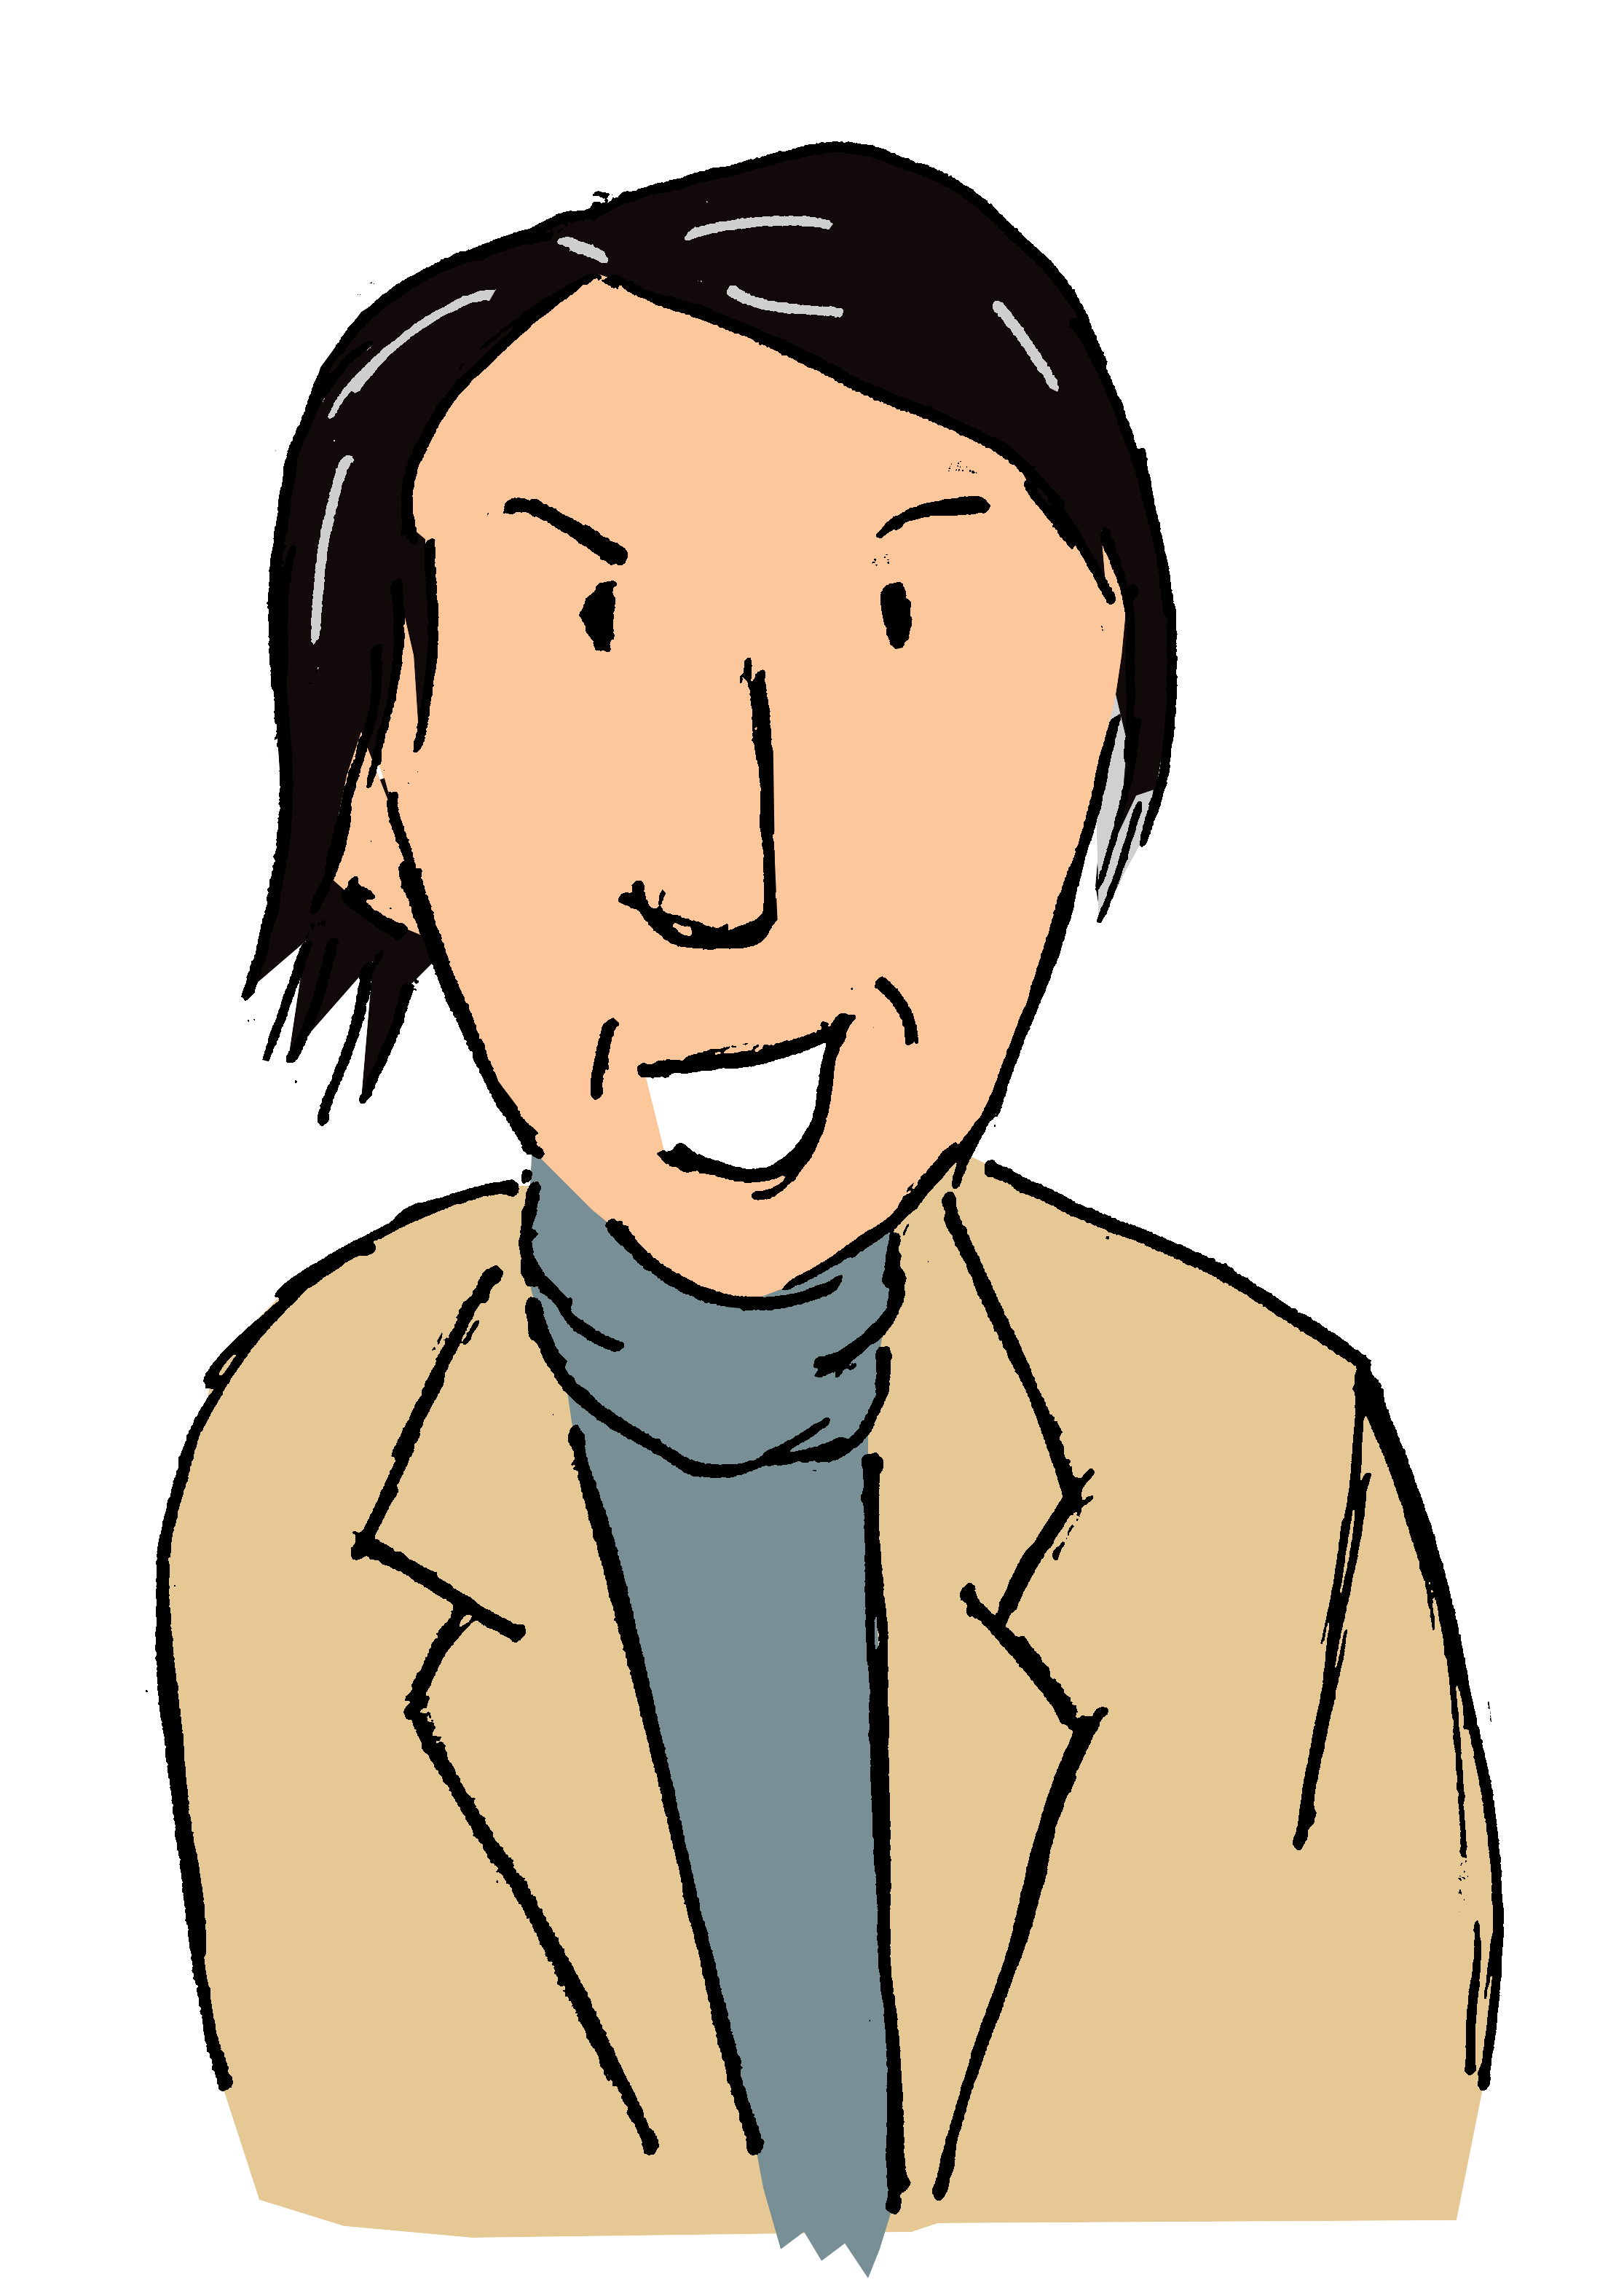
\includegraphics[width=5cm]{img/carl_sagan}};
			\node (example-textwidth-2) [notice={(2.5,0.2)}, ultra thick, right, align=center, text width=14cm, color=black, fill=white, font=\fontsize{23pt}{24pt}\selectfont] at (0,-1) {D'altra parte, dal punto di vista matematico, epicicli e deferenti erano equivalenti a mettere il Sole in movimento intorno alla Terra e gli altri pianeti in movimento intorno al Sole.};
		\end{scope}
		%
		\begin{scope}[shift={(-10,-55)}]
			\node at (0,-2) {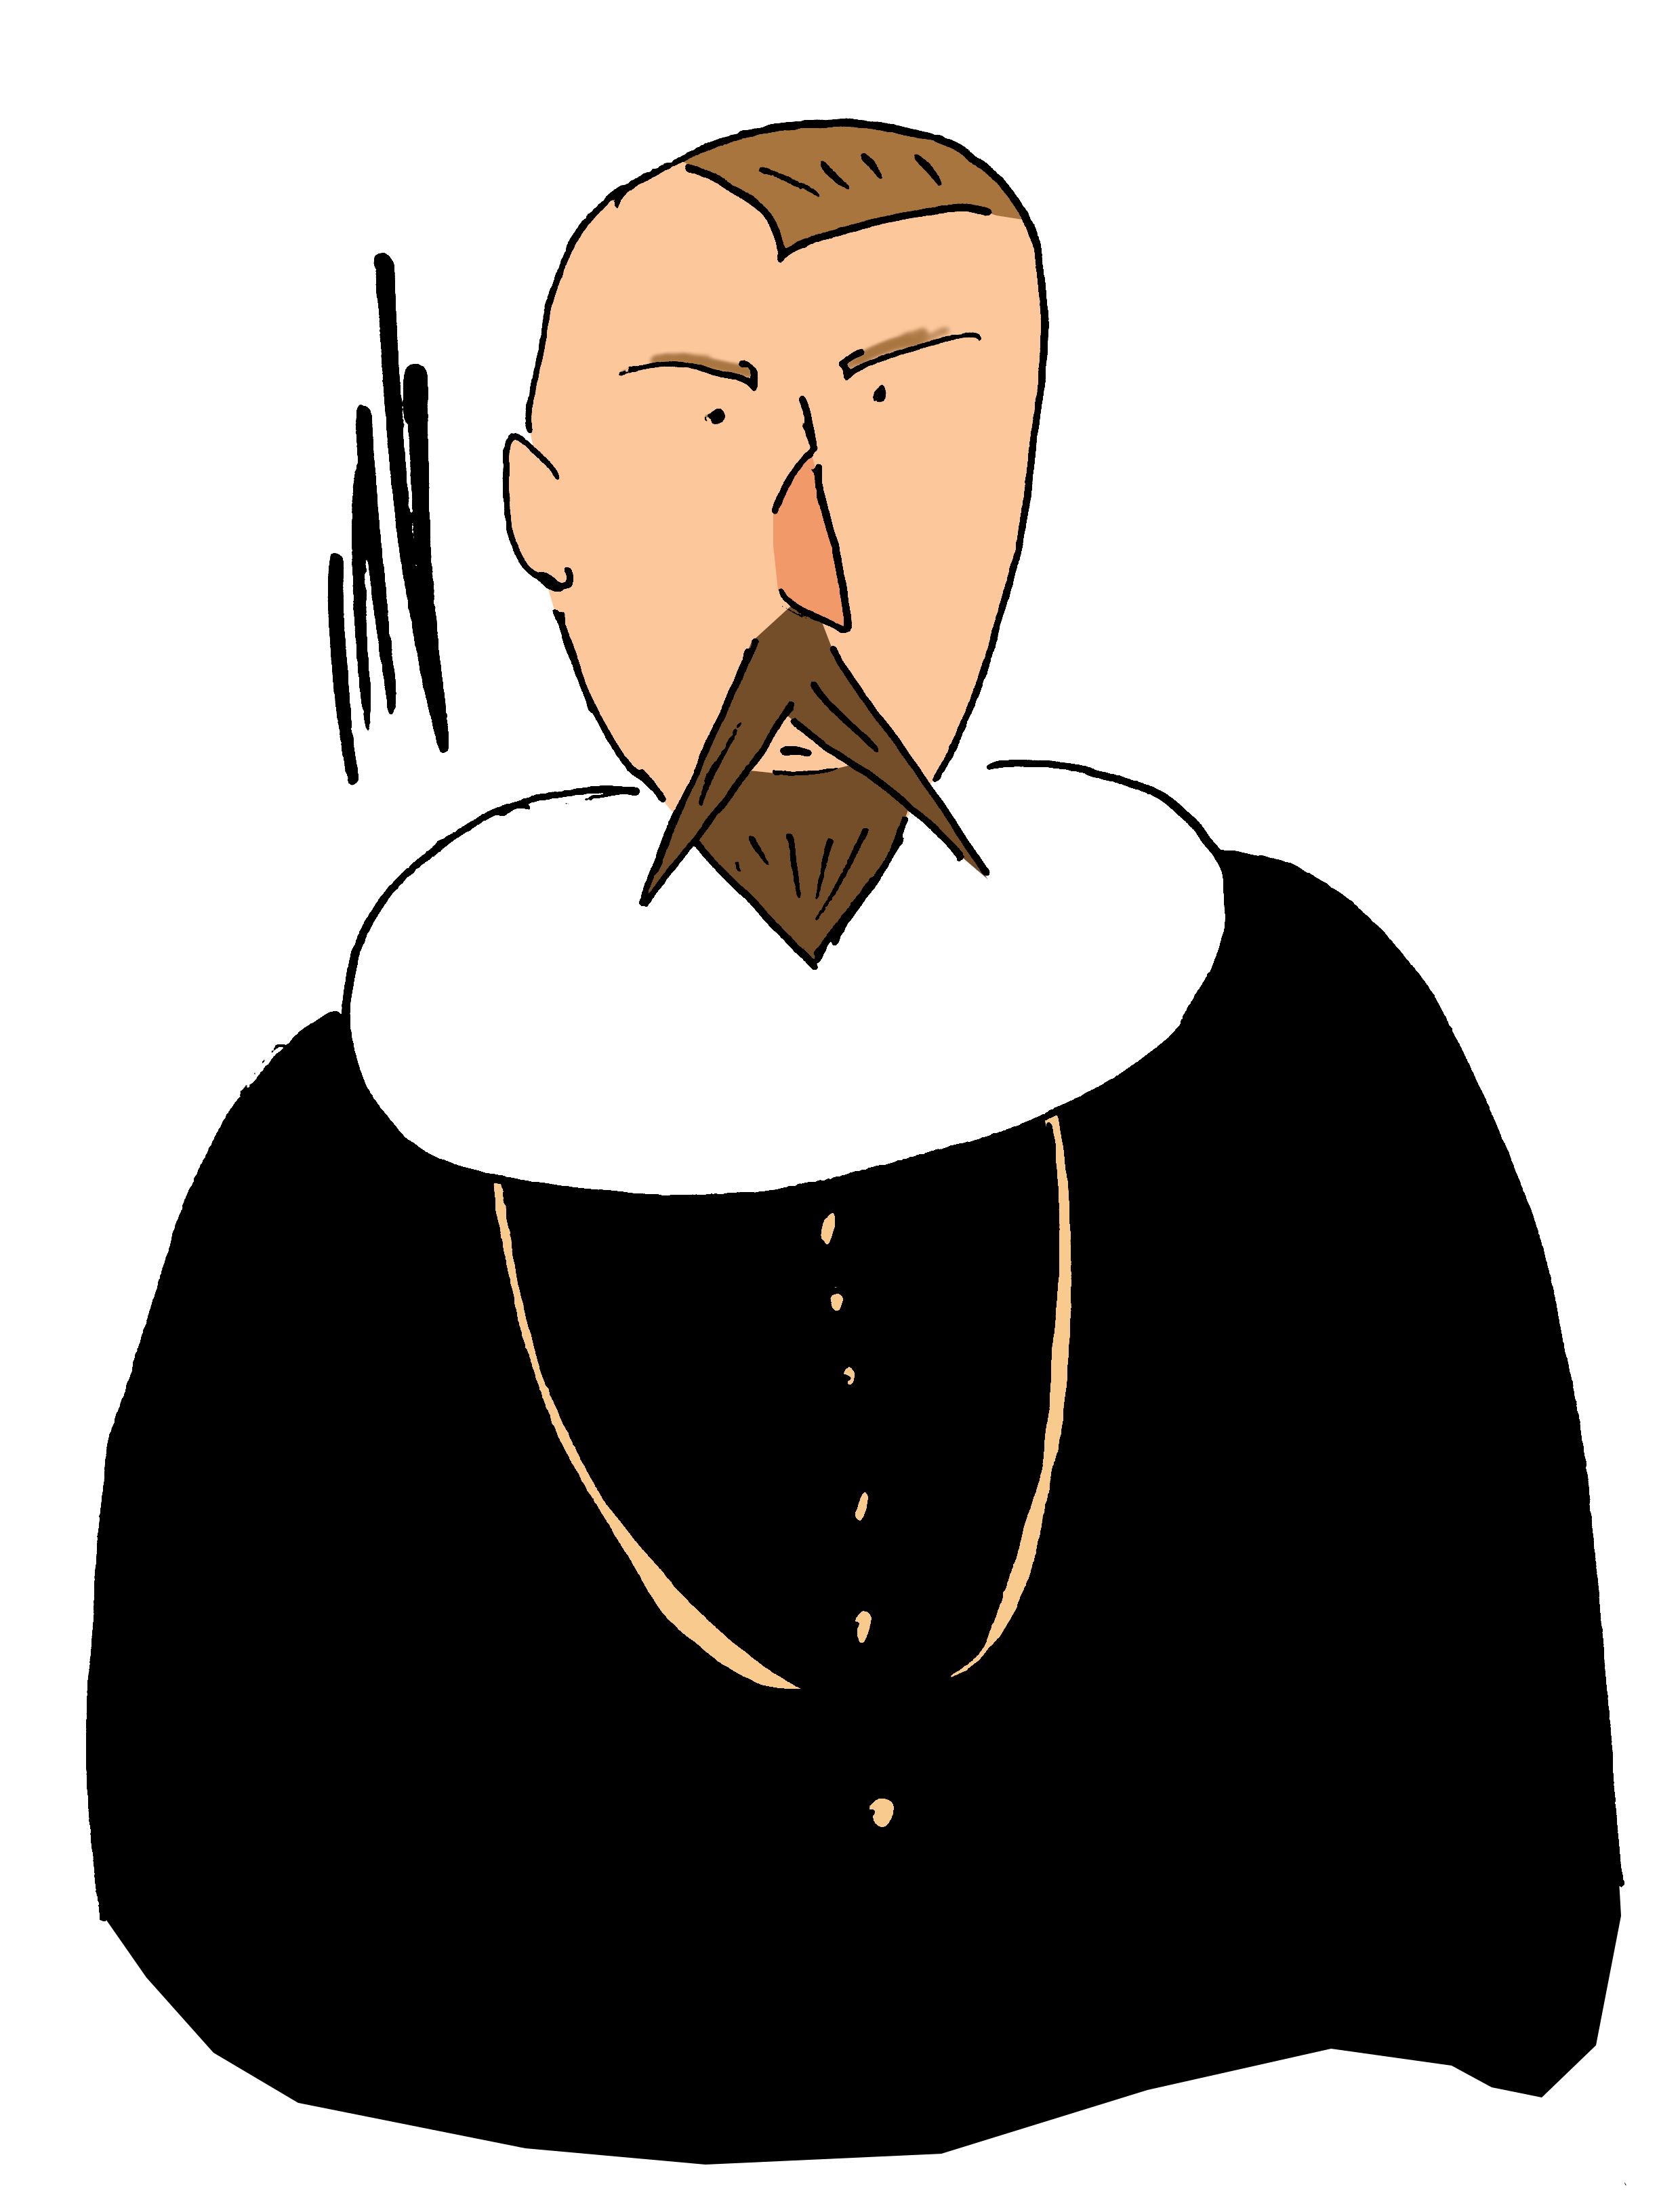
\includegraphics[width=8cm]{img/brahe}};
			\node (example-textwidth-2) [notice={(-3,1)}, ultra thick, right, align=center, text width=12cm, color=black, fill=white, font=\fontsize{23pt}{24pt}\selectfont] at (2,-4.5) {Per me la Terra doveva stare al centro dell'universo! Non riusci' a convincermi del contrario nemmeno il mio miglior allievo, Keplero.};
		\end{scope}
		%
		\begin{scope}[shift={(-10,-68)}]
			\node at (23,0) {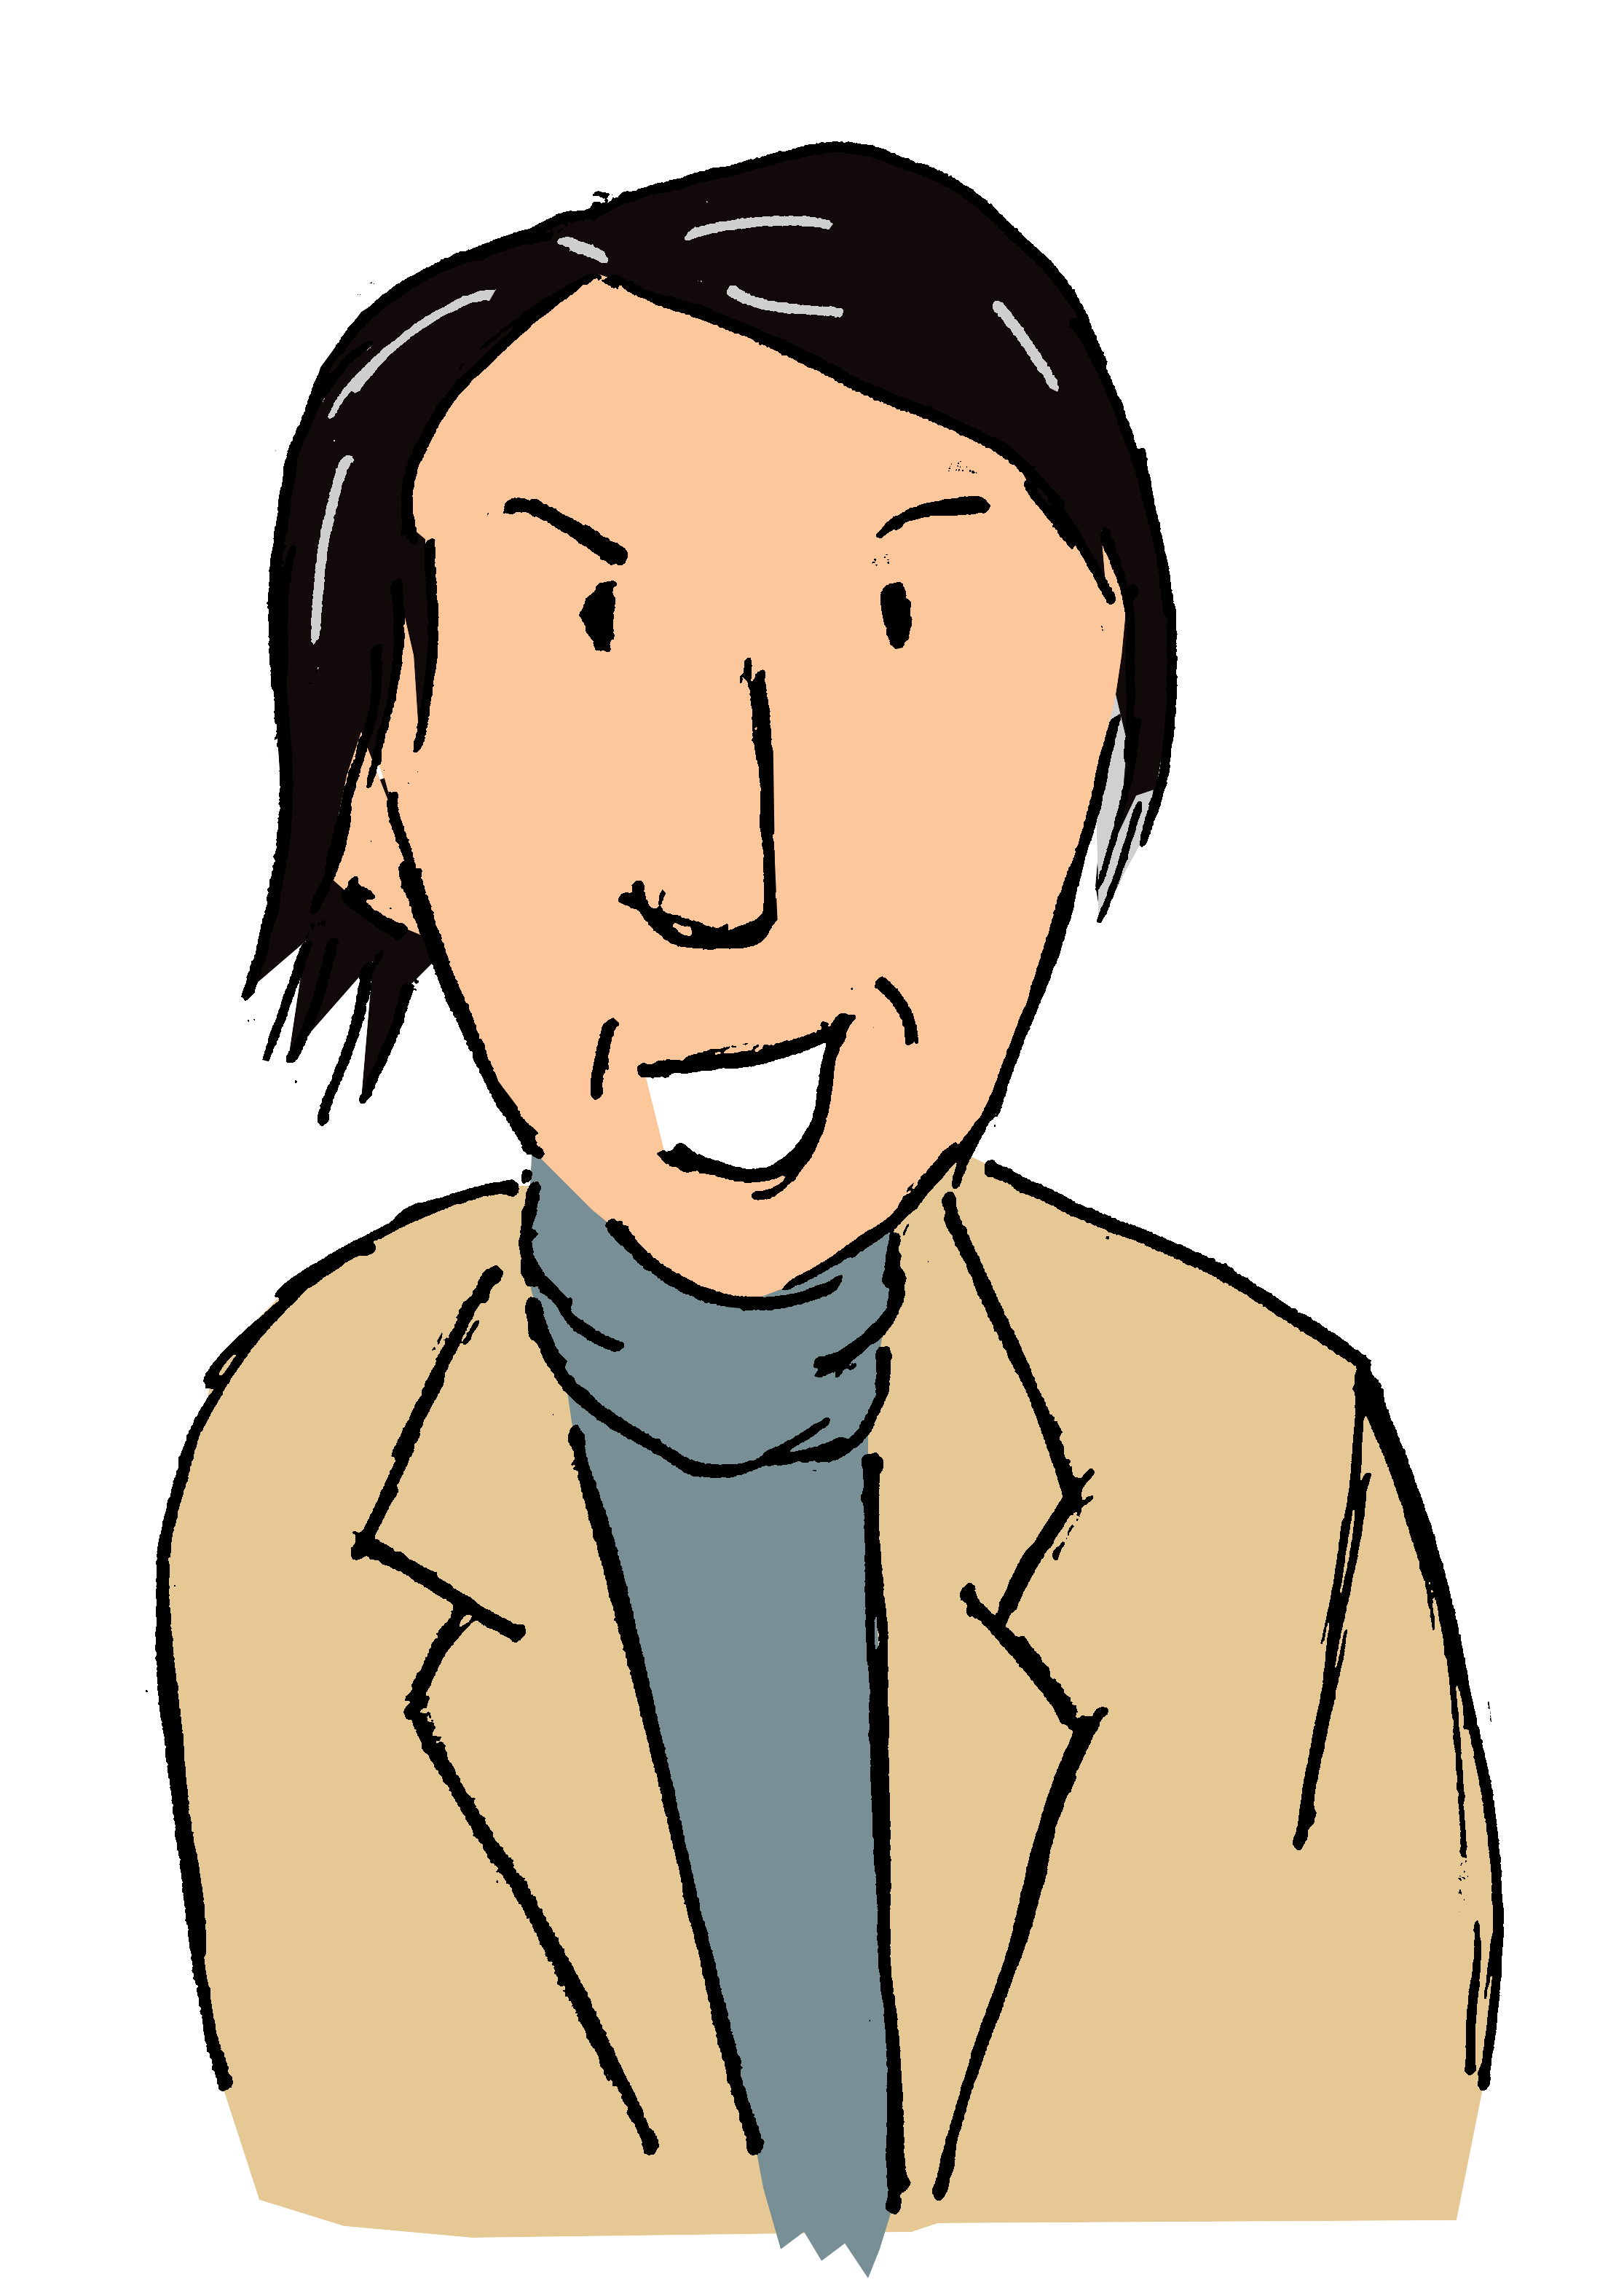
\includegraphics[width=5cm]{img/carl_sagan}};
			\node (example-textwidth-2) [notice={(2.5,0.2)}, ultra thick, right, align=center, text width=15cm, color=black, fill=white, font=\fontsize{23pt}{24pt}\selectfont] at (-1.5,-1) {A proposito delle leggi di Keplero, anche queste potevano essere ricavate a partire dal modello ticonico, giusto per ricordare l'efficacia matematica del modello realizzato dall'astronomo danese.};
		\end{scope}
		%
		\begin{scope}[shift={(-10,-74)}]
			\node at (27,0) () {
\includegraphics[width=3.7cm]{img/licenza}};
			\node at (18,-0.1) {\textcolor{black}{\fontsize{14}{15}\selectfont Testo e illustrazioni: @ulaulaman - Gianluigi Filippelli}};
		\end{scope}
	\end{tikzpicture}
%
\end{document}